\documentclass{article}

\usepackage{graphicx}
\usepackage{tikz}
\usepackage{tikzsymbols}
\usetikzlibrary{calc,patterns,shapes.geometric}
\pagestyle{empty}
\usepackage[margin=0pt]{geometry}
\geometry{papersize={14in,12in}}

\def\centerarc[#1](#2)(#3:#4:#5){\draw[#1] ($(#2)+({#5*cos(#3)},{#5*sin(#3)})$) arc (#3:#4:#5);}

\begin{document}
	\begin{figure}
		\centering
		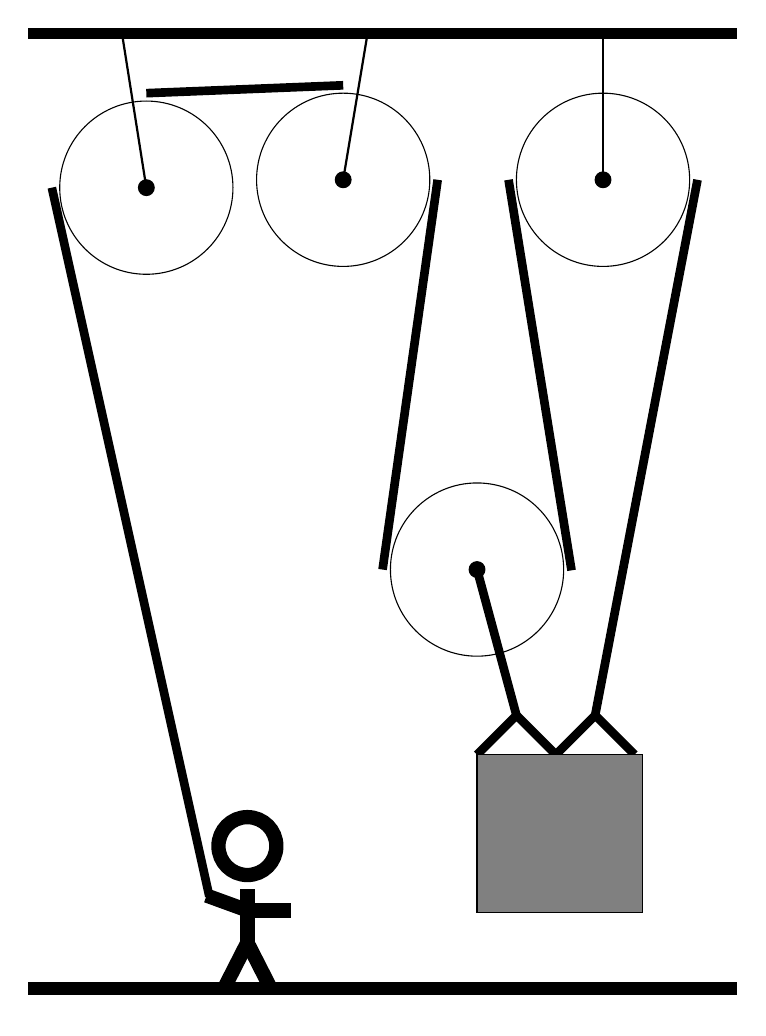
\begin{tikzpicture}
			%%%%% START %%%%%
			\draw[fill=black] (-3, 9) rectangle (6, 9.125);
			
			\draw (1, 7.2) circle (1.1);
			\draw[fill=black] (1, 7.2) circle (0.1);
			\draw[thick] (1, 7.2) -- (1.3, 9);
			
			\draw (4.3, 7.2) circle (1.1);
			\draw[fill=black] (4.3, 7.2) circle (0.1);
			\draw[thick] (4.3, 7.2) -- (4.3, 9);
			
			\draw (2.7, 2.25) circle (1.1);
			\draw[fill=black] (2.7, 2.25) circle (0.1);
			
			\draw[line width=1.1mm]  (2.7, -0.1) -- (3.2, 0.4) -- (3.7, -0.1) -- (4.2, 0.4) -- (4.7, -0.1);
			\draw[fill=black!50] (2.7, -0.1) rectangle (4.8, -2.1);
			
			\draw (-1.5, 7.1) circle (1.1);
			\draw[fill=black] (-1.5, 7.1) circle (0.1);
			\draw[thick] (-1.5, 7.1) -- (-1.8, 9);
			
			\draw[line width=1.1mm](-0.7, -1.9) --  (-2.7, 7.1);
			\centerarc[line width=1.1mm](-1.5, 7.1)(90:180:1.2000000000000002);
			\draw[line width=1.1mm](-1.5, 8.3) -- (1, 8.4);
			\centerarc[line width=1.1mm](1, 7.2)(0:90:1.2000000000000002);
			\draw[line width=1.1mm](2.2, 7.2) -- (1.5, 2.25);
			\centerarc[line width=1.1mm](2.7, 2.25)(180:370:1.2000000000000002);
			\draw[line width=1.1mm] (3.9, 2.24) -- (3.1, 7.2);
			\centerarc[line width=1.1mm](4.3, 7.2)(0:180:1.2000000000000002);
			\draw[line width=1.1mm](4.2, 0.4) -- (5.5, 7.2);
			\draw[line width=1.1mm] (3.2, 0.4) -- (2.7, 2.25);
			
			\node at (-0.2, -2) {\Strichmaxerl[10][-20][0]};
			
			\draw[fill=black] (-3, -3) rectangle (6, -3.15);
			%%%%% END %%%%%
		\end{tikzpicture}
	\end{figure}	
\end{document}